\def\notedate{2023.01.10}
\def\currentauthor{Журавлев Н.В. (РК6-72Б)}
\notestatement{rndhpcedt}{Алгоритмы поиска циклов в ориентированных графах}

Рассматривается ориентированный граф.

Из книги Евстигнеева и Касьянова \flqqГрафы в программировании\frqq\ были рассмотрены и проанализированы следующие алгоритмы~\cite{eg-graph}: 
\begin{enumerate}[label=\arabic*)]
  \item рекурсивный алгоритм обхода графа в глубину;
  \item общий алгоритм обхода графа с запоминанием дуг или вершин;
  \item обход графа в ширину с использованием внешней и внутренней очередей;
  \item обход графа в глубину без использование дополнительной памяти.
\end{enumerate}

Рекурсивный алгоритм обхода графа в глубину (рис.~\ref{fig:rec}а) не желателен для использования, т.к. имеется рекурсия, что может приводить к зацикливанию в процессе обхода, т.к. рассматриваются орграфы. Алгоритм обхода графа в глубину без использование дополнительной памяти (рис.~\ref{fig:rec}б) не подходит, так как для его работы необходим один \flqqприёмник\frqq\messnote{Непонятно ...} из начальной вершины.

\begin{figure}[ht!]
    \centering
\begin{tabular}{P{0.5\textwidth}P{0.5\textwidth}}
  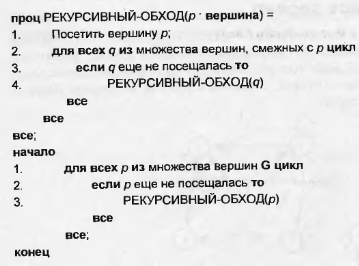
\includegraphics[width=0.4\textwidth]{ResearchNotes/rndhpc_int_edt_2023_01_10/rec.png} &
  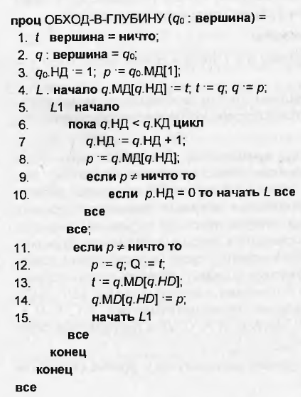
\includegraphics[width=0.4\textwidth]{ResearchNotes/rndhpc_int_edt_2023_01_10/without_memory.png} \\
    а) & б) \\
\end{tabular}
    \caption{Алгоритмы обхода графа в глубину: а)~рекурсивный; б)~без использование дополнительной памяти}\label{fig:rec}
\end{figure}

Общий алгоритм обхода графа с запоминанием дуг (рис.~\ref{fig:save}а) или вершин (рис.~\ref{fig:save}б) имеют одинаковую вычислительную сложность и могут быть применены для рассматриваемого орграфа.\messnote{Надо указать какую. Иначе непонятно что с чем сравнивается.}

\begin{figure}[h!]
    \centering
\begin{tabular}{P{0.5\textwidth}P{0.5\textwidth}}
  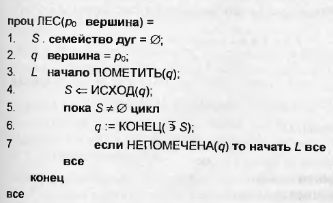
\includegraphics[width=0.4\textwidth]{ResearchNotes/rndhpc_int_edt_2023_01_10/save_arc.png} &
  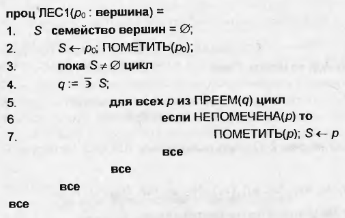
\includegraphics[width=0.4\textwidth]{ResearchNotes/rndhpc_int_edt_2023_01_10/save_eages.png} \\
    а) & б) \\
\end{tabular}
    \caption{Общий алгоритм обхода графа: а)~с запоминанием дуг; б)~с запоминанием вершин}\label{fig:save}
\end{figure}

Алгоритм обхода графа в ширину с использованием внешней очереди (рис.~\ref{fig:queue}а) и алгоритм обхода графа в ширину с использованием внутренней очереди (рис.~\ref{fig:queue}б). Оба алгоритма не подходят, так как имеют \flqqб$\acute{\mbox{о}}$льшую\frqq\ вычислительную сложность, а именно $O(k + t)$, где $k$ и $t$ -- количество дуг и вершин графа, по сравнению с общим алгоритмом обхода графа с запоминанием вершин, сложность которого $O(t)$, где $t$ -- количество дуг, для которого нет зависимости от числа дуг.

\begin{figure}[h!]
    \centering
\begin{tabular}{P{0.5\textwidth}P{0.5\textwidth}}
  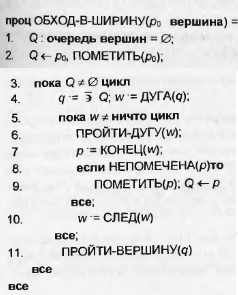
\includegraphics[width=0.4\textwidth]{ResearchNotes/rndhpc_int_edt_2023_01_10/outer_queue.png} &
  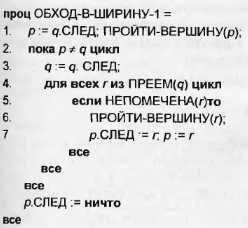
\includegraphics[width=0.4\textwidth]{ResearchNotes/rndhpc_int_edt_2023_01_10/internal_queue.png} \\
    а) & б) \\
\end{tabular}
    \caption{Алгоритмы обхода графа в ширину с использованием: а)~внешней очереди; б)~внутренней очереди}\label{fig:queue}
\end{figure}

\noteattributes{} 